\chapter{The whole project in one picture}
\label{ch:bigpicture}

\section{The project in five sentences}

\begin{enumerate}
  \item You built a benchmark of \textbf{366 forest patches} (each about 640\,m across) in the Kanha Tiger Reserve region of Madhya Pradesh, each seen in two matched dry seasons: \textbf{T0 = January--February 2022} and \textbf{T1 = January--February 2023}.
  \item For every patch you collected \textbf{five data sources} (Sentinel-2 optical, Sentinel-1 radar, CHIRPS rainfall, ERA5-Land climate anomalies, NASADEM terrain), made a before/after pair of colour images and a text \textbf{evidence card}, and gave it an automatic label: \texttt{decline}, \texttt{stable} or \texttt{increase}, from the change in NDVI.
  \item You tested \textbf{four small open vision--language models} on the same 55 test patches. With the full card, whose last line states the label, Qwen2-VL-2B reached \textbf{56.4\,\%} and the other three 32.7--36.4\,\%. With that line removed, Qwen fell to \textbf{32.7\,\%} and LLaVA reached 43.6\,\%: no model beats always guessing one class (34.5\,\%).
  \item A small \textbf{LoRA fine-tune} of Qwen2-VL-2B on 16 balanced training patches with the label-free card reached \textbf{36.4\,\%}, answering ``stable'' for almost everything. An earlier, unbalanced run with the full card (67.3\,\%) is superseded.
  \item When the models had to \textbf{justify} their answers with the label removed, free-form text was unreliable; a \textbf{structured ``cite-only'' prompt} made 71--76\,\% of checkable claims agree with the measurements, and a pilot \textbf{explanation LoRA} on 16 self-generated justifications reached 61.8\,\% class accuracy but only 50.5\,\% correct claims.
\end{enumerate}

\section{The research question and what kind of project this is}

The research roadmap (\file{EcoExplain-VLM_Complete_Research_Roadmap.pdf}, Section~1) states the central question:

\begin{quote}
\emph{Can vision--language models correctly classify forest vegetation change and generate explanations that are supported by multimodal remote-sensing and climate evidence?}
\end{quote}

The question has two halves, and the project has two halves to match: \textbf{classification} (Tracks~A and~B) and \textbf{explanation} (Track~C).

\begin{plainwords}
EcoExplain-VLM is an \emph{evaluation benchmark}, not a new remote-sensing model. You did not try to beat existing forest-change maps. You built a fixed test, put existing general-purpose models through it, and measured carefully what they could and could not do. A clear negative or mixed result is a valid outcome for a benchmark, as long as it is measured honestly.
\end{plainwords}

\section{Your workflow figure, box by box}

Figure~\ref{fig:workflow-yours} is the workflow figure you made for your report (\file{papers/acl/fig_workflow.png}). It is the map for the whole guide: each numbered stage has its own chapter.

\begin{figure}[H]
\centering
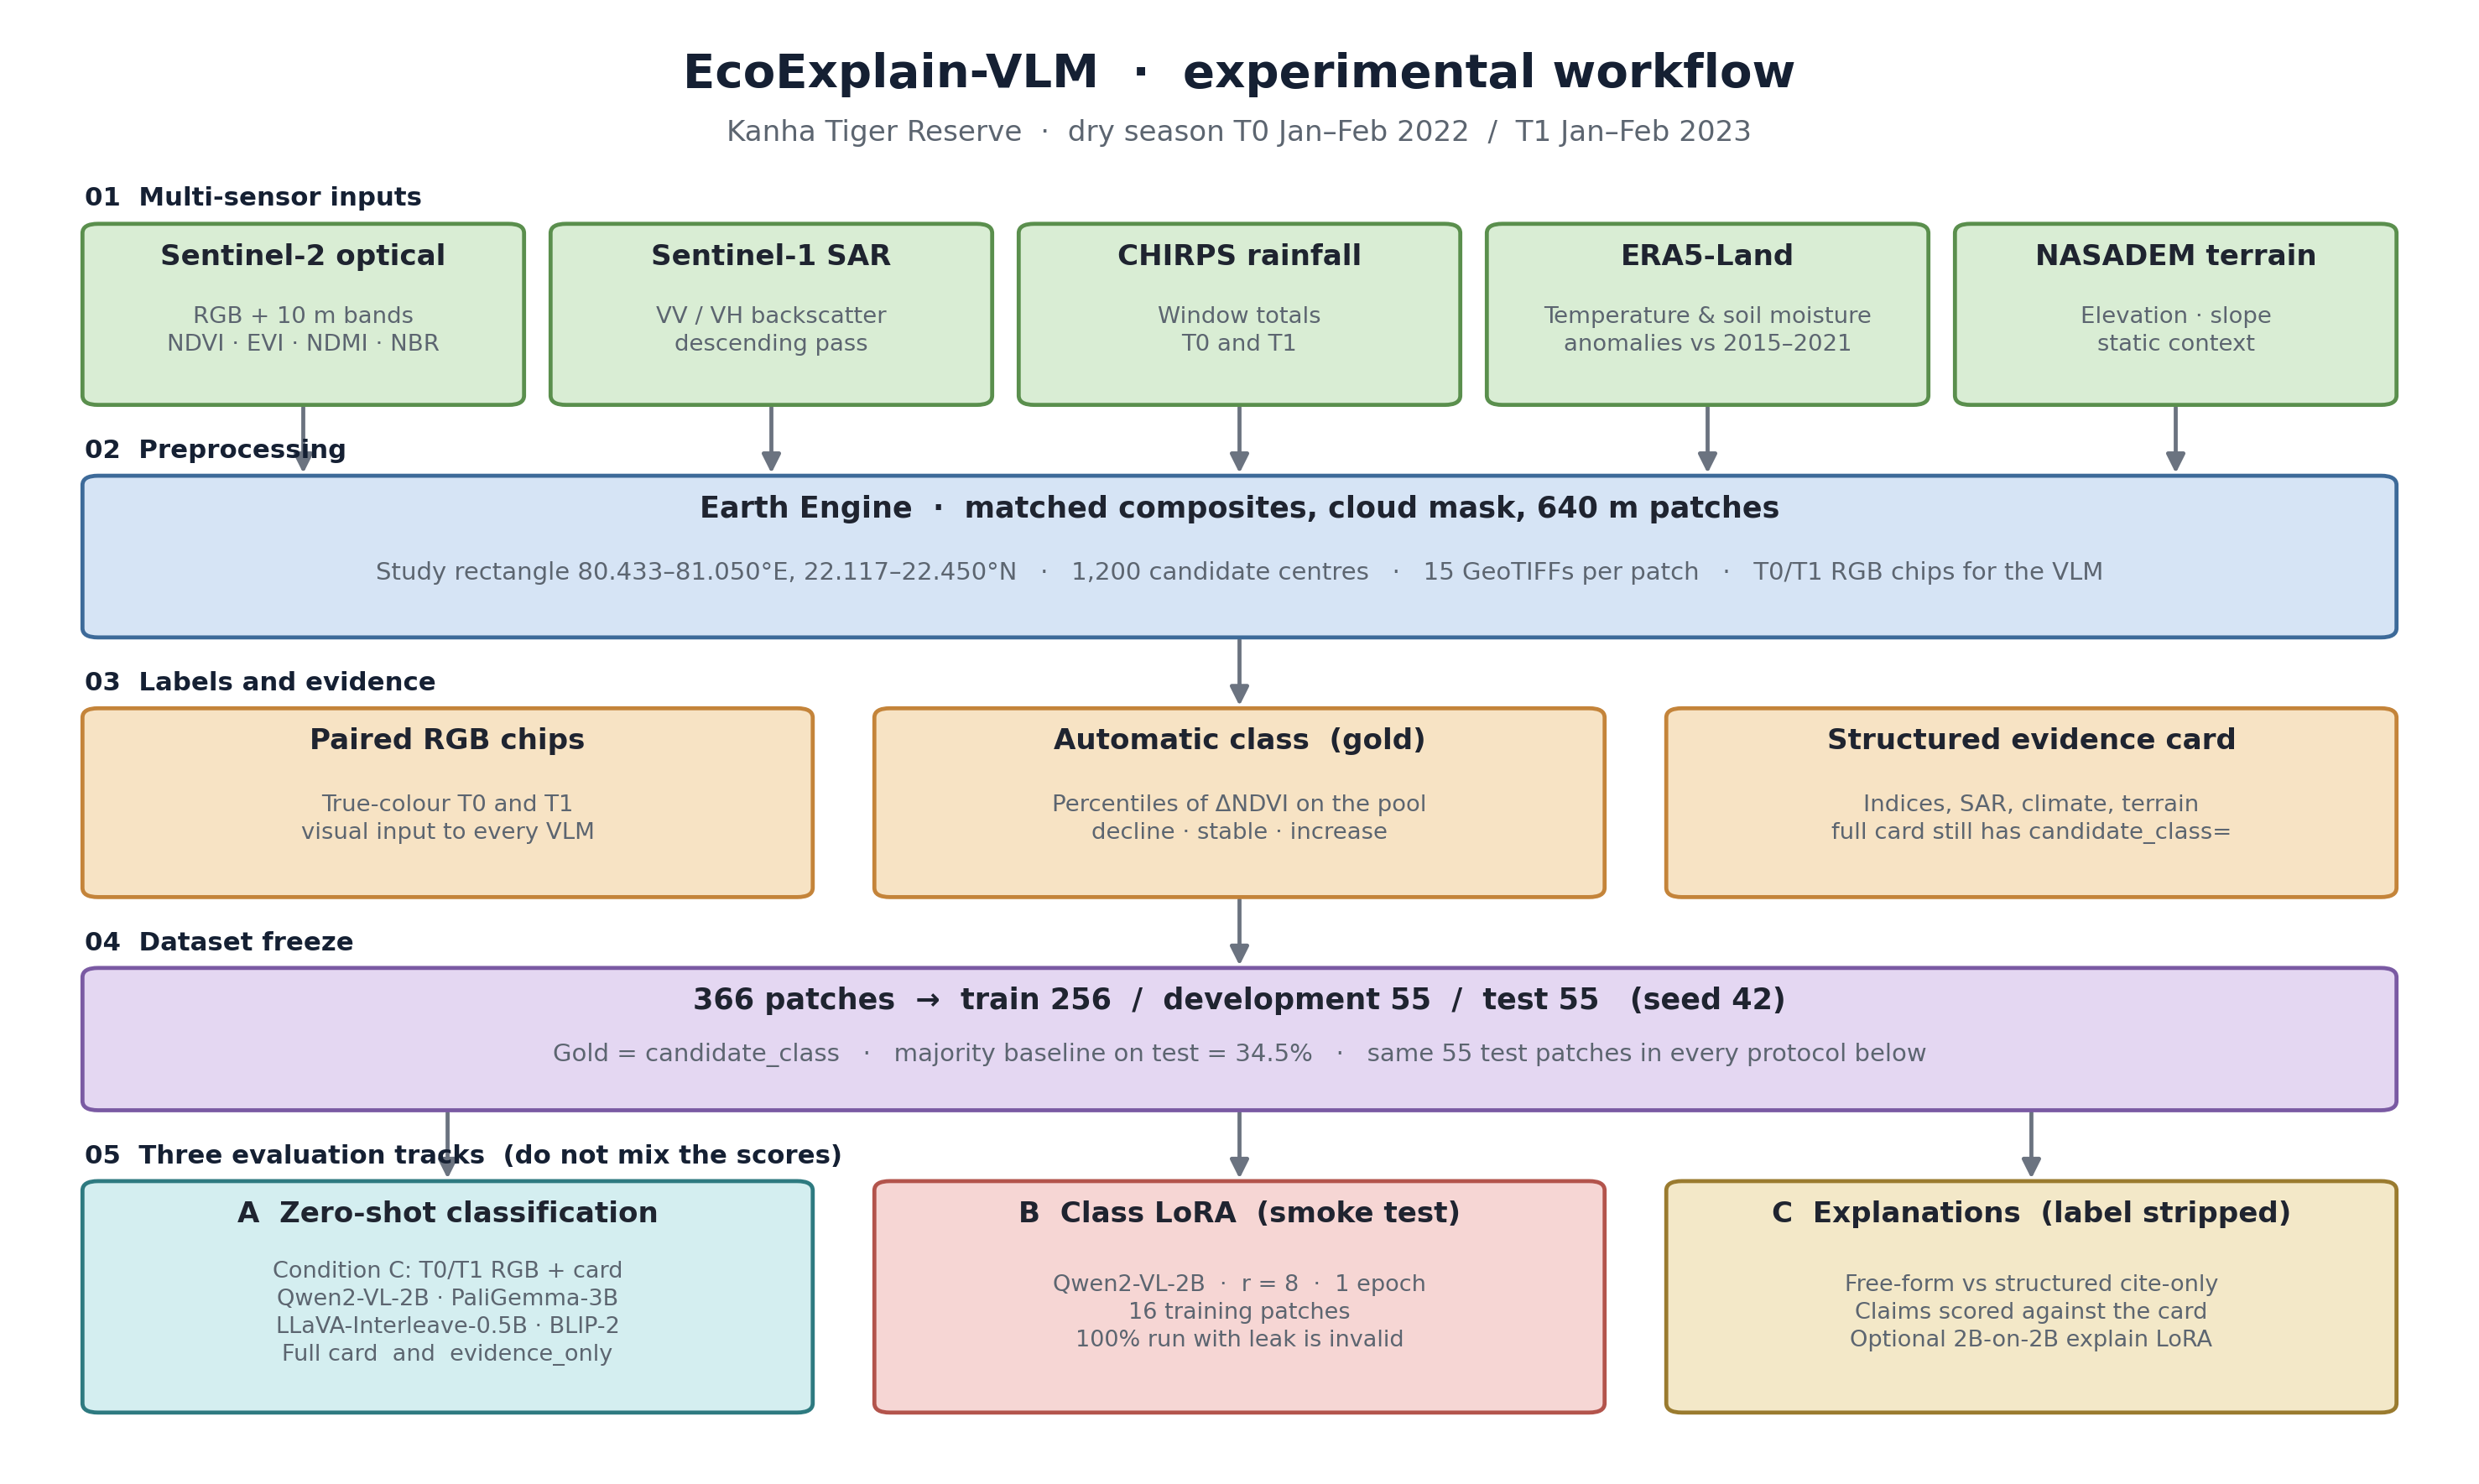
\includegraphics[width=\textwidth]{figures/fig_workflow_yours.png}
\caption{Your workflow figure, as it is now (\file{papers/acl/fig_workflow.png}, made by \file{papers/acl/make_workflow_figure.py}). Two box texts in stage~05 need correcting; Chapter~\ref{ch:figures} explains why and shows a corrected copy.}
\label{fig:workflow-yours}
\end{figure}

\begin{longtable}{L{2.6cm}L{8.2cm}L{3.0cm}}
\caption{What each stage of the workflow means, and where the guide explains it.}\label{tab:stages}\\
\toprule
\textbf{Stage} & \textbf{What happens} & \textbf{Guide} \\
\midrule
\endfirsthead
\toprule
\textbf{Stage} & \textbf{What happens} & \textbf{Guide} \\
\midrule
\endhead
01 Multi-sensor inputs & Five sources describe each place: what the canopy looks like and how green it is (Sentinel-2), its structure and wetness (Sentinel-1), rain (CHIRPS), temperature and soil moisture compared with normal (ERA5-Land), and terrain (NASADEM). & Chapter~\ref{ch:stage01} \\
02 Preprocessing & Google Earth Engine combines all images of each two-month window into one cloud-free picture per year, cuts 640\,m patches around candidate centres, and exports 15 files per patch. Image processing then makes 512\,$\times$\,512 colour chips and arrays. & Chapter~\ref{ch:stage02} \\
03 Labels and evidence & Three things come out for every patch: a pair of colour images (T0, T1), an automatic label from the NDVI change, and a text evidence card listing the measured values. & Chapter~\ref{ch:stage03} \\
04 Dataset freeze & The 366 records are frozen in \file{dataset.jsonl} and split once into 256 training, 55 development and 55 test patches. Always predicting the most common test class scores 34.5\,\%. & Chapter~\ref{ch:stage04} \\
05 Three evaluation tracks & A: four models classify the test patches without training. B: one model is fine-tuned with LoRA and tested again. C: the models are asked to justify their answers, and their claims are checked against the measurements. & Chapters~\ref{ch:trackA}--\ref{ch:trackC} \\
\bottomrule
\end{longtable}

\begin{watchout}
Two things in the figure are not accurate, and both matter because the figure will be one of the first things your professor looks at:
\begin{itemize}
  \item Track~A says every model received ``T0/T1 RGB + card''. Only Qwen2-VL-2B and LLaVA-Interleave-0.5B did. PaliGemma received one NDVI line, and BLIP-2 one stitched image with no evidence text.
  \item Track~A lists ``Full card and evidence\_only'' as if all four models were run both ways. The \texttt{evidence\_only} re-run covered three models on all 55 patches and Qwen on only 3, and it changed the input of LLaVA only.
\end{itemize}
Chapter~\ref{ch:figures} gives the exact lines to change in \file{make_workflow_figure.py} and a corrected copy.
\end{watchout}

\section{The order in which the work happened: four phases}

The work did not happen in the neat order of the figure. It happened in four phases, each prompted by what the previous one showed (Figure~\ref{fig:phases}).

\begin{figure}[H]
\centering
\begin{tikzpicture}[
  box/.style={draw, rounded corners=3pt, align=left, font=\small, inner sep=5pt, text width=3.25cm, minimum height=2.3cm},
  prep/.style={box, fill=green!6},
  pha/.style={box, fill=orange!8},
  phb/.style={box, fill=gray!10},
  phc/.style={box, fill=blue!7},
  phd/.style={box, fill=red!6},
  arr/.style={-{Stealth[length=2.2mm]}, thick, gray!70!black}
]
\node[prep] (plan) {\textbf{Plan}\\ 29 Jun--8 Aug\\ roadmap, handbook,\\ work order};
\node[prep, right=0.5cm of plan] (pilot) {\textbf{Pilot}\\ 3--7 Sep\\ 36 patches checked\\ by a person};
\node[prep, right=0.5cm of pilot] (data) {\textbf{Dataset}\\ 16--24 Sep\\ 372 exported, 366\\ kept; split frozen};
\node[pha, below=0.9cm of plan] (A) {\textbf{Phase A}\\ 25 Sep--2 Oct\\ zero-shot (Track A)\\ class LoRA (Track B)};
\node[phb, right=0.5cm of A] (B) {\textbf{Phase B}\\ 2--3 Oct\\ free-form\\ explanations};
\node[phc, right=0.5cm of B] (C) {\textbf{Phase C}\\ 6 Oct\\ structured cite-only\\ explanations};
\node[phd, right=0.5cm of C] (D) {\textbf{Phase D}\\ 16--17 Oct\\ explanation LoRA\\ on Ada};
\node[box, fill=teal!8, below=0.7cm of D] (E) {\textbf{Phase E}\\ 19--20 Oct\\ leak-free reruns,\\ balanced LoRA};
\draw[arr] (plan) -- (pilot);
\draw[arr] (pilot) -- (data);
\draw[arr] (data.south) -- ++(0,-0.45) -| (A.north);
\draw[arr] (A) -- (B);
\draw[arr] (B) -- (C);
\draw[arr] (C) -- (D);
\draw[arr] (D) -- (E);
\end{tikzpicture}
\caption{The order of the work in 2026. Dates come from file times, notebook outputs, Slurm logs and the git history; the first guide (\file{study_guide/}, Chapter~3) has the day-by-day timeline.}
\label{fig:phases}
\end{figure}

\begin{table}[H]
\centering
\caption{Phases (when the work happened) against tracks (how your workflow figure groups the experiments).}
\label{tab:phasetrack}
\small
\begin{tabularx}{\textwidth}{lYY}
\toprule
Phase & What it did & Track in your figure \\
\midrule
A & Four models classify the 55 test patches; Qwen2-VL-2B fine-tuned with LoRA on 16 patches; supporting runs (label line removed, closed-set probe, threshold baselines) & Track~A (zero-shot) and Track~B (class LoRA) \\
B & Models asked to explain their answer in their own words (``free-form'' or ``legacy'' prompt) & Track~C, first part \\
C & Models asked to copy listed facts and follow a stated rule (``structured cite-only'' prompt) & Track~C, second part \\
D & Qwen2-VL-2B fine-tuned on 16 of its own filtered explanations (``explanation LoRA'') & Track~C, third part \\
E & Protocol fixes and reruns: Qwen and LLaVA without the summary line; balanced, label-free class LoRA; parser fix; spatial split & Track~A (leak-free rows) and Track~B (new run) \\
\bottomrule
\end{tabularx}
\end{table}

\begin{foryourreport}
Pick one naming scheme for the report and keep to it. The tracks of your figure are the clearer choice for a Methods section, because they describe experiments rather than dates. If you keep the letters A/B/C for tracks, do not also call the explanation prompts ``Phase B'' and ``Phase C'' in the same report, or a reader will confuse Track~B (class LoRA) with Phase~B (free-form explanations). Descriptive names avoid the problem: ``zero-shot classification'', ``class LoRA'', ``free-form explanations'', ``structured explanations'', ``explanation LoRA''.
\end{foryourreport}

\section{What was found, in one paragraph per track}

\paragraph{Track A, zero-shot classification.} With the full card, Qwen2-VL-2B was correct on 31 of 55 test patches (56.4\,\%); PaliGemma-3B scored 36.4\,\%, LLaVA-Interleave-0.5B and BLIP-2 OPT-2.7B 32.7\,\% each, the level of always predicting one class (the majority baseline is 34.5\,\%). Removing the summary line dropped Qwen to 32.7\,\% (a significant drop, $p = 0.011$), and with the same label-free table for every model LLaVA reached 43.6\,\% (not significantly above the baseline). A one-number rule on the evidence card's \dndvi{} value, with two cut-offs fitted on the training split, scores 94.5\,\%: the card holds enough information, but the small models do not extract it.

\paragraph{Track B, class LoRA.} The reported run (Ada job 29575) fine-tuned Qwen2-VL-2B on 16 class-balanced training patches with the label-free card, for one epoch: 36.4\,\% (20 of 55), answering ``stable'' for 53 patches. The first run (16 patches chosen by ID, full card) reached 67.3\,\% but read the card's label line and never answered ``stable''; longer full-card runs reached 100\,\%. Both are superseded.

\paragraph{Track C, explanations.} With a free-form prompt, PaliGemma and BLIP-2 gave no checkable reasons and LLaVA's claims were right 56.7\,\% of the time. A structured prompt that lists allowed facts and states an NDVI rule raised claim correctness to 75.8\,\% (Qwen) and 71.1\,\% (LLaVA), but the answers mostly restate the given facts, and Qwen's class simply follows the stated rule. The explanation LoRA reached 61.8\,\% class accuracy with 50.5\,\% correct claims, worse on claims than structured prompting.

\section{The numbers to know by heart}

\begin{longtable}{L{6.0cm}L{3.0cm}L{5.2cm}}
\caption{Twelve numbers that carry the report. Appendix~\ref{app:facts} has the full list.}\label{tab:heart}\\
\toprule
\textbf{Quantity} & \textbf{Value} & \textbf{Source file} \\
\midrule
\endfirsthead
\toprule
\textbf{Quantity} & \textbf{Value} & \textbf{Source file} \\
\midrule
\endhead
Study rectangle & 80.433--81.050\dg E, 22.117--22.450\dg N; 2,350.7\,km$^2$ & \file{configs/pilot_kanha.yaml}; notebook 01 \\
Windows & T0 Jan--Feb 2022; T1 Jan--Feb 2023 & \file{configs/pilot_kanha.yaml} \\
Patches & 1,200 candidates $\rightarrow$ 366 final (120 / 124 / 122) & \file{data/raw_metadata/composite_stats.csv}, \file{dataset.jsonl} \\
Label cut-offs & $q_{15} = -0.0377$, $q_{85} = +0.0031$ & computed from the 1,200-patch pool \\
Split & 256 / 55 / 55, seed 42; test 18 / 18 / 19 & \file{data/splits/split_manifest.json} \\
Majority baseline & 34.5\,\% (19/55) & same \\
Human check & 8 of 19 agree (42\,\%) & \file{results/preflight_report.json} \\
Zero-shot, full card (Track A) & Qwen 56.4\,\%; PaliGemma 36.4\,\%; LLaVA 32.7\,\%; BLIP-2 32.7\,\% & \file{results/vlm_combo_*.json} \\
Zero-shot, leak-free (Track A) & Qwen 32.7\,\% (\texttt{evidence\_only} and \texttt{compact}); LLaVA 43.6\,\% (\texttt{compact}) & \file{results/protocol/} \\
Class LoRA (Track B) & 36.4\,\% (balanced 16, label-free, Ada job 29575); old 67.3\,\% superseded & \file{results/protocol/qwen_balanced_leakfree_lora.json} \\
Threshold baseline & 94.5\,\% (fitted on train); 63.6\,\% ($\pm0.02$) & \file{study_guide_v3/build_results_master.py} \\
Structured explanations & 75.8\,\% (Qwen), 71.1\,\% (LLaVA) correct claims & \file{results/explain/explanation_scores.csv} \\
Explanation LoRA & 61.8\,\% class accuracy; 50.5\,\% correct claims; 28/256 kept, 16 used & \file{results/explain/explanation_scores.json}, \file{target_filter_report.json} \\
\bottomrule
\end{longtable}

\section{Five things the report must say clearly}

These five statements protect the whole report. An examiner who finds any of them missing will doubt the rest.

\begin{enumerate}
  \item \textbf{What the full card contains.} Every evidence card ends with the pipeline's summary line, which includes the trend word and \texttt{candidate\_class}, the same field used as the gold label. Qwen's 56.4\,\% (and the old 67.3\,\%) were obtained with that card (Chapter~\ref{ch:trackA}).
  \item \textbf{What happens without it.} Qwen falls to 32.7\,\%; no model beats the 34.5\,\% baseline without the line. This is now your central classification finding, not a footnote.
  \item \textbf{What each model received.} Qwen and LLaVA: both images and the full card. PaliGemma: both images and one NDVI line. BLIP-2: one stitched image and a short prompt (Table~\ref{tab:inputs}).
  \item \textbf{How small the fine-tunes were.} Every LoRA run reported used 16 training examples for one epoch. Say this every time 36.4\,\% or 61.8\,\% appears.
  \item \textbf{What the labels are.} Relative ranks of NDVI change inside this region and pair of years, checked by one person on 19 patches with 42\,\% agreement. They are not a validated map of forest disturbance.
\end{enumerate}

\begin{whybox}
Stating these does not weaken the report; it fixes what the numbers mean. ``Qwen2-VL-2B reached 56.4\,\% with the full card and 32.7\,\% without its summary line'' is a clear, honest finding about what small VLMs actually use. Reporting 56.4\,\% alone would turn a true number into a misleading one.
\end{whybox}

\begin{selfcheck}
\begin{enumerate}
  \item In one sentence each, what happens in stages 01, 02, 03, 04 and 05 of your workflow?
  \item What is the difference between Phase~B and Track~B?
  \item Why is 34.5\,\%, and not 33.3\,\%, the number to compare models against?
  \item Which two models saw the full evidence card in Track~A?
  \item Name the five things the report must say clearly.
\end{enumerate}
\end{selfcheck}
